\documentclass{beamer}
\usepackage[utf8]{inputenc}
\usepackage[T1]{fontenc}
% \usepackage{amscd, amsfonts, amsmath, amssymb, amstext, amsthm, caption, epsfig, fancyhdr, float, graphicx, latexsym, mathtools, multicol, multirow, algorithm, chngcntr}
\usepackage[english, french]{babel}
\usepackage{booktabs}

\usepackage{amsmath,amssymb}
\usepackage{graphicx}
\usepackage{caption}
\usepackage{subfig}
\usepackage{xspace}
\usepackage{fourier}


\usepackage{tikz}
\usetikzlibrary{shapes,arrows}
\usepackage{tkz-graph}
\usetikzlibrary{automata,arrows,positioning,calc}
\usetikzlibrary{positioning}
\usetikzlibrary{fit}
\usetikzlibrary{backgrounds}
\usetikzlibrary{calc}
\usetikzlibrary{shapes}
\usetikzlibrary{mindmap}
\usetikzlibrary{decorations.text}
\usetikzlibrary{snakes}

% \theoremstyle{definition} % insert bellow all blocks you want in normal text
% \newtheorem{definition}{Definition}



% tikzmark command, for shading over items
\newcommand{\tikzmark}[1]{\tikz[overlay,remember picture] \node (#1) {};}
% Define block styles
\tikzstyle{decision} = [diamond, draw, fill=blue!20,
    text width=4.5em, text badly centered, node distance=3cm, inner sep=0pt]
\tikzstyle{block} = [rectangle, draw, fill=blue!20,
    text width=5em, text centered, rounded corners]
\tikzstyle{line} = [draw]
\tikzstyle{cloud} = [draw, ellipse,fill=red!20, node distance=3cm,
    minimum height=2em]

\usepackage[most]{tcolorbox}

\setbeamertemplate{blocks}[rounded][shadow=true] % use rounded blocks with standard beamer shadow


% Distributions.
\newcommand*{\UnifDist}{\mathsf{Unif}}
\newcommand*{\ExpDist}{\mathsf{Exp}}
\newcommand*{\DepExpDist}{\mathsf{DepExp}}
\newcommand*{\GammaDist}{\mathsf{Gamma}}
\newcommand*{\LognormalDist}{\mathsf{LogNorm}}
\newcommand*{\WeibullDist}{\mathsf{Weib}}
\newcommand*{\ParetoDist}{\mathsf{Par}}
\newcommand*{\NormalDist}{\mathsf{Norm}}

\newcommand*{\GeometricDist}{\mathsf{Geom}}
\newcommand*{\NegBinomialDist}{\mathsf{NegBin}}
\newcommand*{\PoissonDist}{\mathsf{Poisson}}
\newcommand*{\BivariatePoissonDist}{\mathsf{BPoisson}}
\newcommand*{\CyclicalPoissonDist}{\mathsf{CPoisson}}

\newcommand*{\iid}{\textbf{iid}\@\xspace}
\newcommand*{\pdf}{\textbf{pdf}\@\xspace}
\newcommand*{\cdf}{\textbf{cdf}\@\xspace}
\newcommand*{\pmf}{\textbf{pmf}\@\xspace}
\newcommand*{\abc}{{\textbf{abc}}\@\xspace}
\newcommand*{\smc}{\textbf{smc}\@\xspace}
\newcommand*{\mcmc}{\textbf{mcmc}\@\xspace}
\newcommand*{\ess}{\textbf{ess}\@\xspace}
\newcommand*{\mle}{\textbf{mle}\@\xspace}
\newcommand*{\bic}{\textbf{bic}\@\xspace}
\newcommand*{\kde}{\textbf{kde}\@\xspace}
\newcommand*{\glm}{\textbf{glm}\@\xspace}
\newcommand*{\xol}{\textbf{xol}\@\xspace}
\newcommand*{\cpu}{\textbf{cpu}\@\xspace}
\newcommand*{\gpu}{\textbf{gpu}\@\xspace}
\newcommand*{\arm}{\textbf{arm}\@\xspace}

\def \si {\sigma}
\def \la {\lambda}
\def \al {\alpha}
% \def\e*{\end{eqnarray*}}
\def \di{\displaystyle}

\def \E{\mathbb E}
\def \N{\mathbb N}
\def \Z{\mathbb Z}
\def \NZ{\mathbb{N}_0}
\def \I{\mathbb I}
\def \w{\widehat}
\def \P {\mathbb P}
\def \V{\mathbb V}


\newcommand{\CL}{\mathbb{C}}
\newcommand{\RL}{\mathbb{R}}
\newcommand{\nat}{{\mathbb N}}
\newcommand{\Laplace}{\mathscr{L}}
\newcommand{\e}{\mathrm{e}}
\newcommand{\ve}{\bm{\mathrm{e}}} % vector e

\renewcommand{\L}{\mathcal{L}} % e.g. L^2 loss.

\newcommand{\ih}{\mathrm{i}}
\newcommand{\oh}{{\mathrm{o}}}
\newcommand{\Oh}{{\mathcal{O}}}
\newcommand{\Exp}{\mathbb{E}}

\newcommand{\Norm}{\mathcal{N}}
\newcommand{\LN}{\mathcal{LN}}
\newcommand{\SLN}{\mathcal{SLN}}

\renewcommand{\Pr}{\mathbb{P}}
\newcommand{\Ind}{\mathbb I}
\newcommand\bfsigma{\bm{\sigma}}
\newcommand\bfSigma{\bm{\Sigma}}
\newcommand\bfLambda{\bm{\Lambda}}
\newcommand{\stimes}{{\times}}
\def \limsup{\underset{n\rightarrow+\infty}{\overline{\lim}}}
\def \liminf{\underset{n\rightarrow+\infty}{\underline{\lim}}}




% vertical separator macro
\newcommand{\vsep}{
  \column{0.0\textwidth}
    \begin{tikzpicture}
      \draw[very thick,black!10] (0,0) -- (0,7.3);
    \end{tikzpicture}
}
\newcommand\blfootnote[1]{%
  \begingroup
  \renewcommand\thefootnote{}\footnote{#1}%
  \addtocounter{footnote}{-1}%
  \endgroup
}

% More space between lines in align
% \setlength{\mathindent}{0pt}

% Beamer theme
\usetheme{ZMBZFMK}
\usefonttheme[onlysmall]{structurebold}
\mode<presentation>
\setbeamercovered{transparent=10}

% align spacing
\setlength{\jot}{0pt}

\setbeamertemplate{navigation symbols}{}%remove navigation symbols

\title[BLOCKASTICS]{Blockchain, bitcoins and decentralized finance}
% \subtitle{Introduction}
\author{Pierre-O. Goffard}
\institute[IRMA]{UNISTRA\\
 \texttt{goffard@unistra.fr}
}
\date{\today}
% \titlegraphic{\includegraphics[width=2.5cm]{../../Figures/bfs_logo.png}} 

\begin{document}
\begin{frame}
  \titlepage
\end{frame}
\begin{frame}{Outline}
  \tableofcontents
\end{frame}

\section{Introduction}
\begin{frame}{Blockchain}
A data ledger made of a sequence of blocks maintained by a achieving consensus in a Peer-To-Peer network.
\begin{columns}
\begin{column}{0.5\textwidth}
% \small

\begin{itemize}
  \item Decentralized
  \item Public/private
  \item Permissionned/permissionless
  \item Immutable
  \item Incentive compatible
\end{itemize}
\end{column}
\begin{column}{0.5\textwidth}
\begin{center}
\begin{tikzpicture}[-, >=stealth', auto, semithick, node distance=01cm]
\tikzstyle{every edge}=[snake=expanding waves,segment length=1mm,segment angle=10, draw]

\tikzstyle{full node}=[circle, fill=tublue,draw=tublue,thick,text=black,scale=0.8]
\tikzstyle{light node}=[circle, fill=white,draw=tublue,thick,text=black,scale=0.8]
\node[full node]    (1)                     {};
\node[full node]    (2)[above right of=1]         {};
\node[full node]    (3)[above left of=1]         {};
\node[full node]    (4)[below of=1]         {};
\node[full node]    (5)[right of=4]         {};
\node[full node]    (6)[below of=4]         {};
\node[light node]    (7)[left of=1]         {};
\node[light node]    (8)[right of=2]         {};
\node[light node]    (9)[left of=4]         {};
\node[light node]    (10)[above right of=5]         {};
\node[light node]    (11)[ right of=5]         {};
\node[light node]    (12)[ below right of=5]         {};
% \node[light node]    (4)[above of=2]         {};
\path

(1) edge node{} (2)
    edge node{} (3)
    edge node{} (7)
    ;
\path
(5) edge node{} (10)
    edge node{} (11)
    edge node{} (12)
    ;
    \path
(4) edge node{} (5)
    edge node{} (1)
    edge node{} (9)
    edge node{} (6)
    ;
    \path
(2) edge node{} (8)   
    ;
\end{tikzpicture}
\end{center}
\end{column}
\end{columns}

\vspace{0.2cm}
We will focus on public blockchain and their associated consensus protocol.
\end{frame}
\begin{frame}{Blocks}
A block contains
\begin{itemize}
  \item block height/ID
  \item Time stamp
  \item hash of the block
  \item hash of the previous block
  \item Set of transactions (data stored in the blockchain)
\end{itemize}
\begin{center}
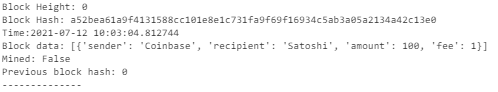
\includegraphics[width=0.9\textwidth]{../../Figures/genesis_block.png}
\end{center}
\url{https://www.blockchain.com/}
\end{frame}
% \begin{frame}{Cryptographic Hash function}
% \small
% A function that maps data of arbitratry size (message) to a bit array of fixed size (hash value)
% $$
% h:\{0,1\}^\ast\mapsto \{0,1\}^d. 
% $$
% A good hash function is
% \begin{itemize}
% \item deterministic
% \item quick to compute
% \item One way
% \begin{itemize}
%   \scriptsize
% \item[$\hookrightarrow$] For a given hash value $\overline{h}$ it is hard to find a message $m$ such that 
% $$
% h(m) = \overline{h}
% $$
% \end{itemize}
% \item Colision resistant 
% \begin{itemize}
% \item[$\hookrightarrow$] Impossible to find $m_1$ and $m_2$ such that 
% $$
% h(m_1) = h(m_2)
% $$
% \end{itemize}
% \item Chaotic
% $$m_1\approx m_2\Rightarrow  h(m_1) \neq h(m_2)$$
% \end{itemize}

% \end{frame}
\begin{frame}{Consensus protocols}
The mechanism to make all the nodes agree on a common data history.\\
\vspace{0.3cm}
The three dimensions of blockchain systems analysis
\begin{enumerate}
  \item Efficiency 
  \begin{itemize}
    \item Throughputs
    \item Transaction confirmation time
  \end{itemize}
  \item Decentralization 
  \begin{itemize}
    \item Fair distribution of the accounting right
  \end{itemize}
  \item Security 
  \begin{itemize}
    \item Resistance to attacks
  \end{itemize}
\end{enumerate}
\footnotesize
\begin{thebibliography}{1}
\bibitem{Fu2020}
X.~Fu, H.~Wang, and P.~Shi, ``A survey of blockchain consensus algorithms:
  mechanism, design and applications,'' {\em Science China Information
  Sciences}, vol.~64, nov 2020.
\end{thebibliography}
\end{frame}
% \begin{frame}{Proof of Work}
% The nodes compete to solve a cryptographic problem by brute force search.
% \begin{tcolorbox}[enhanced,drop shadow, title=PoW]
% \begin{enumerate}
%     \item Draw a random number (nonce)
%     \[
%     X\sim\{1,\ldots, 2^{32}\}.
%     \]
%     \item While $X > L$, where $L$ is the target then try again  
% \end{enumerate}
% \end{tcolorbox}
% \vspace{0.3cm}
% Nodes are chosen according to their computing power
% {\footnotesize
% \begin{thebibliography}{1}
% \bibitem{Na08}
% S.~Nakamoto, ``Bitcoin: A peer-to-peer electronic cash system.'' Available at
%   \href{https://bitcoin.org/bitcoin.pdf}{https://bitcoin.org/bitcoin.pdf},
%   2008.
% \end{thebibliography}  
% }
% \end{frame}
% \begin{frame}{Proof of Stake}
% PoW is slow and ressource consuming. Let $\{1,\ldots, N\}$ be a set of miner and $\{\pi_1,\ldots, \pi_N\}$ be their share of cryptocoins.
% \begin{tcolorbox}[enhanced,drop shadow, title=PoS]
% Node $i\in \{1,\ldots, N\}$ is selected with probability $\pi_i$ to append the next block
% \end{tcolorbox}
% \vspace{0.3cm}
% Nodes are chosen according to what they own.
% \begin{itemize}
%   \item Nothing at stake problem
%   \item Rich gets richer ? (To be discussed later on)
% \end{itemize}
% \footnotesize{
% \begin{thebibliography}{1}

% \bibitem{Saleh2020}
% F.~Saleh, ``Blockchain without waste: Proof-of-stake,'' {\em The Review of
%   Financial Studies}, vol.~34, pp.~1156--1190, jul 2020.

% \end{thebibliography}}

% \end{frame}
\begin{frame}{Applications of blockchain: Cryptocurrency}
\begin{columns}
\begin{column}{0.5\textwidth}
   
{\footnotesize
\begin{thebibliography}{1}
\bibitem{Na08}
S.~Nakamoto, ``Bitcoin: A peer-to-peer electronic cash system.'' Available at
  \href{https://bitcoin.org/bitcoin.pdf}{https://bitcoin.org/bitcoin.pdf},
  2008.
  \bibitem{Antonopoulos2017}
A.~Antonopoulos, {\em Mastering Bitcoin}.
\newblock O'Reilly UK Ltd., July 2017.
\end{thebibliography}  
}
\end{column}
\begin{column}{0.5\textwidth}  %%<--- here
    \begin{center}
     
\includegraphics[width=0.5\textwidth]{../../Figures/bitcoin-6284869_1920.png}
     \end{center}
\end{column}
\end{columns}

\begin{itemize}
  \item Transaction anonymity
  \item Banking and reliable currency in certain regions of the world
  \item Money Transfer worldwide (at low fare)
  \item No need for a thrusted third party
\end{itemize}
\end{frame}
\section{Consensus protocol}
\begin{frame}{Consensus protocol}
\begin{tcolorbox}[enhanced,drop shadow, title=Definition]
    Algorithm to allows the full nodes to agree on a common data history
\end{tcolorbox}
It must rely on the scarce resources of the network
\begin{itemize}
  \item bandwidth
  \item computational power
  \item storage (disk space)
\end{itemize}
\end{frame}
\begin{frame}{Types of consensus protocols}
\begin{enumerate}
  \item Voting based 
  \footnotesize
\begin{thebibliography}{1}

\bibitem{lamport1982the}
L.~Lamport, R.~Shostak, and M.~Pease, ``The byzantine generals problem,'' {\em
  ACM Transactions on Programming Languages and Systems}, pp.~382--401, July
  1982.

\end{thebibliography}
\normalsize
\begin{itemize}
  \item[\danger] Communication overhead
  \item[\danger] Denial of service
\end{itemize}

  \item Leader based
  \begin{itemize}
    \item Proof-of-Work (computational power)
    \item Proof-of-Capacity and Proof-of-Spacetime (storage)
    \item Proof-of-Interaction (bandwidth)
    \item Proof-of-Stake (tokens)
  \end{itemize}
\end{enumerate}
\end{frame}
\begin{frame}{Conflict resolution in blockchain}
\begin{tcolorbox}[enhanced,drop shadow, title=Fork]
    A fork arises when there is a disagreement between the nodes resulting in several branches in the blockchain.
\end{tcolorbox}
\begin{tcolorbox}[enhanced,drop shadow, title=LCR]
    The \textit{Longest Chain Rule} states that if there exist several branches of the blockchain then the longest should be trusted.
\end{tcolorbox}
In practice 
\begin{itemize}
  \item A branch can be considered legitimate if it is $k\in\mathbb{N}$ blocks ahead of its pursuers.
  \item Fork can be avoided when
  $$
  \text{block appending time}> \text{ propagation delay} 
  $$
\end{itemize}
\end{frame}
\begin{frame}{Proof-of-Work}
\begin{tcolorbox}[enhanced,drop shadow, title=Objective]
    Elect a leader based on computational effort to append the next block.
\end{tcolorbox}
\end{frame}
\begin{frame}{What's inside a block?}
A block consists of 
\begin{itemize}
\item a header 
\item a list of "transactions" that represents the information recorded through the blockchain. 
\end{itemize}
The header usually includes 
\begin{itemize}
\item the date and time of creation of the block, 
\item the block height which is the index inside the blockchain, 
\item the hash of the block 
\item the hash of the previous block. 
\end{itemize}
\begin{tcolorbox}[enhanced,drop shadow, title=Question]
What is the hash of a block?
\end{tcolorbox}
\end{frame}
\begin{frame}{Cryptographic Hash function}
\small
A function that maps data of arbitratry size (message) to a bit array of fixed size (hash value)
$$
h:\{0,1\}^\ast\mapsto \{0,1\}^d. 
$$
A good hash function is
\begin{itemize}
\item deterministic
\item quick to compute
\item One way
\begin{itemize}
  \scriptsize
\item[$\hookrightarrow$] For a given hash value $\overline{h}$ it is hard to find a message $m$ such that 
$$
h(m) = \overline{h}
$$
\end{itemize}
\item Colision resistant 
\begin{itemize}
\item[$\hookrightarrow$] Impossible to find $m_1$ and $m_2$ such that 
$$
h(m_1) = h(m_2)
$$
\end{itemize}
\item Chaotic
$$m_1\approx m_2\Rightarrow  h(m_1) \neq h(m_2)$$
\end{itemize}
\end{frame}
\begin{frame}{SHA-256}
The SHA-256 function which converts any message into a hash value of $256$ bits.
\begin{tcolorbox}[enhanced,drop shadow, title=Example]
The hexadecimal digest of the message
$$
\texttt{BLOCKASTICS is fantastic!}
$$
is 
\footnotesize
$$
\texttt{60a147c28568dc925c347bce20c910ef90f3774e2501ac63344f3411b6a6bf79}
$$
\end{tcolorbox}
\end{frame}
\begin{frame}{Hidden prediction}
\begin{center}
 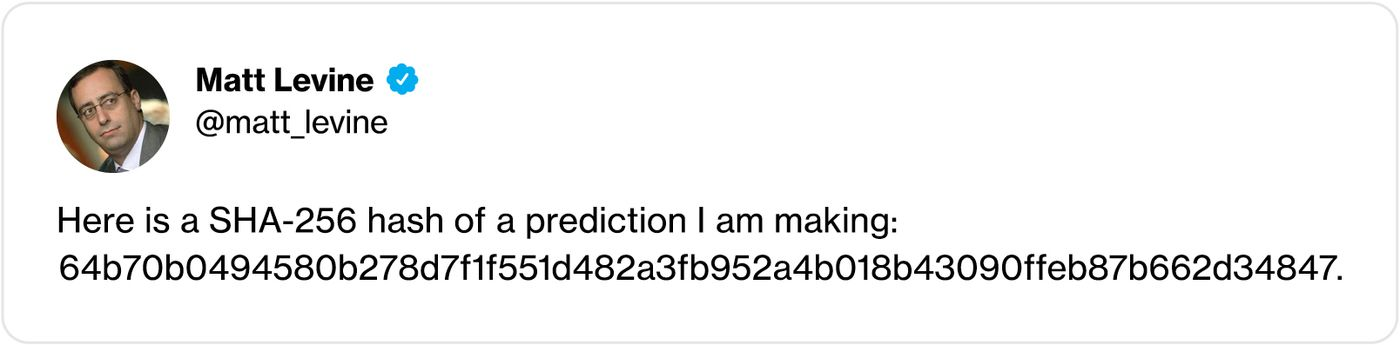
\includegraphics[width= \textwidth]{../../Figures/levine_twitter}
\end{center}
\footnotesize{
\begin{thebibliography}{1}
\bibitem{levine}
M.~Levine, ``The crypto story.'' Bloomberg business week, Oct. 2022.\\
\end{thebibliography}  
}




\end{frame}
\begin{frame}{Mining a block}
\begin{figure}[!ht]
    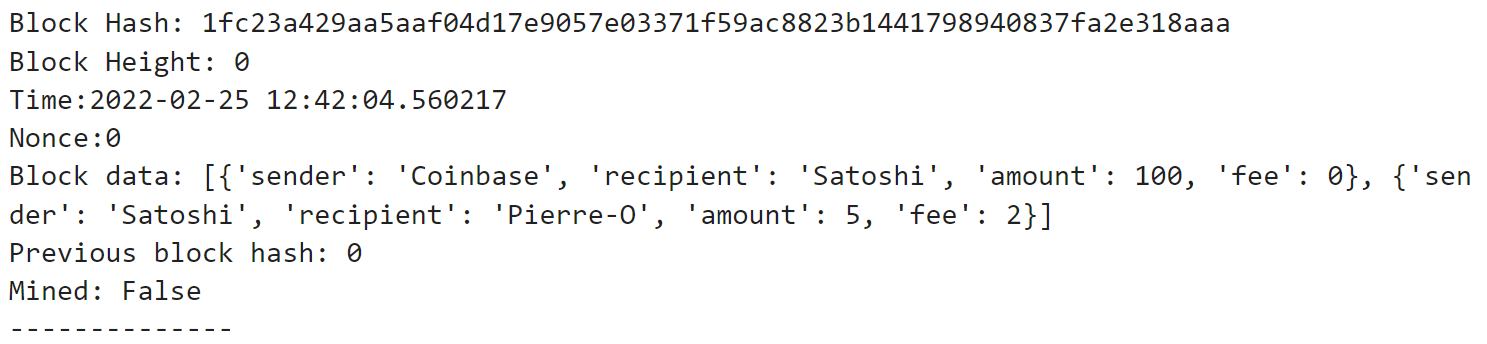
\includegraphics[width = \textwidth]{../../Figures/block_not_mined.png}
    \captionsetup{width=0.8\textwidth}
    \centering
    \caption{A block that has not been mined yet.}
    \label{fig:block_not_mined}
\end{figure}
\end{frame}
\begin{frame}{Mining a block}
The maximum value for a 256 bits number is
$$
T_\text{max} = 2^{256}-1 \approx 1.16e^{77}.
$$
Mining consists in drawing at random a nonce 
$$
\text{Nonce} \sim \text{Unif}(\{0,\ldots, 2^{32}-1\}),
$$
until 
$$
h(\text{Nonce}|\text{Block info})<T,
$$
where $T$ is referred to as the target.
\begin{tcolorbox}[enhanced,drop shadow, title=Difficulty of the cryptopuzzle]
$$
D = \frac{T_{\max}}{T}.
$$
\end{tcolorbox}

\end{frame}
\begin{frame}{Mining a block}
If we set the difficulty to $D = 2^4$ then the hexadecimal digest must start with at least $1$ leading $0$
\begin{figure}[!ht]
    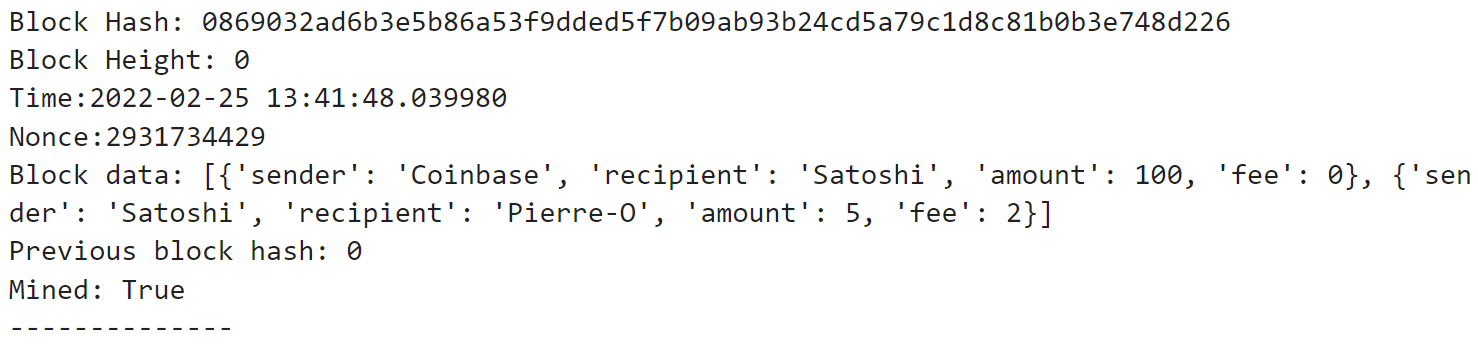
\includegraphics[width = \textwidth]{../../Figures/block_mined.png}
    \captionsetup{width=0.8\textwidth}
    \centering
    \caption{A mined block with a hash value having on leading zero.}
    \label{fig:block_mined}
\end{figure}
The number of trial is geometrically distributed
\begin{itemize}
\item Exponential inter-block times
\item Lenght of the blockchain = Poisson process
\end{itemize}
\end{frame}
\begin{frame}{Bitcoin protocol}
\begin{itemize}
  \item One block every 10 minutes on average
  \item Depends on the hashrate of the network
  \item Difficulty adjustment every 2,016 blocks ($\approx$ two weeks)
  \item Reward halving every 210,000 blocks
\end{itemize}
Check out \url{https://www.bitcoinblockhalf.com/}
\end{frame}
\begin{frame}{Mining equipments}
How it started
\begin{itemize}
  \item CPU, GPU
\end{itemize}
How it is going
\begin{itemize}
  \item Application Specific Integrated Chip (ASIC)
  \begin{itemize}
  \item Increase of the network electricity consumption \url{https://digiconomist.net/bitcoin-energy-consumption}
  \item E-Waste
  \item Centralization issue \url{https://www.bitmain.com/}
  \begin{itemize}
    \item Mining pool ranking at \url{https://btc.com/}
    \item Mining equipment profitability at \url{https://v3.antpool.com/minerIncomeRank}
  \end{itemize}
  \end{itemize}
\end{itemize}
\end{frame}

\begin{frame}{Proof of Stake}
PoW is slow and ressource consuming. Let $\{1,\ldots, N\}$ be a set of miners and $\{\pi_1,\ldots, \pi_N\}$ be their share of cryptocoins.
\begin{tcolorbox}[enhanced,drop shadow, title=PoS]
\begin{enumerate}
\item Node $i\in \{1,\ldots, N\}$ is selected with probability $\pi_i$ to append the next block
\end{enumerate}
\end{tcolorbox}
\vspace{0.3cm}
Nodes are chosen according to what they own.
\begin{itemize}
  \item Nothing at stake problem
  \item Rich gets richer ? 
  \item \url{https://www.peercoin.net/}
\end{itemize}
\footnotesize{
\begin{thebibliography}{1}
\bibitem{Saleh2020}
F.~Saleh, ``Blockchain without waste: Proof-of-stake,'' {\em The Review of
  Financial Studies}, vol.~34, pp.~1156--1190, jul 2020.
\end{thebibliography}}
\end{frame}
\begin{frame}{Incentive mechanism}
Participation to the network is costly to the nodes.


\begin{tcolorbox}[enhanced,drop shadow, title= Native cryptocurrency]
The nodes must be retributed for their hard work.
\end{tcolorbox}

\end{frame}

\section{Cryptocurrencies and decentralized finance}
\begin{frame}{Applications of blockchain: Cryptocurrency}
\begin{columns}
\begin{column}{0.5\textwidth}
   
{\footnotesize
\begin{thebibliography}{1}
\bibitem{Na08}
S.~Nakamoto, ``Bitcoin: A peer-to-peer electronic cash system.'' Available at
  \href{https://bitcoin.org/bitcoin.pdf}{https://bitcoin.org/bitcoin.pdf},
  2008.
\end{thebibliography}  
}
\end{column}
\begin{column}{0.5\textwidth}  %%<--- here
    \begin{center}
     
\includegraphics[width=0.5\textwidth]{../../Figures/bitcoin-6284869_1920.png}
     \end{center}
\end{column}
\end{columns}

\begin{itemize}
  \item Transaction anonymity
  \item Banking and reliable currency in certain regions of the world
  \item Money Transfer worldwide (at low fare)
  \item No need for a thrusted third party
\end{itemize}
\end{frame}
\begin{frame}{Why cryptocurrencies?}
What is wrong with the current financial system?
\begin{itemize}
  \item No data privacy
  \item No real ownership
  \item Outdated technology to transfer ownersip
  \item Huge middlemen costs
\end{itemize}
\scriptsize
\begin{thebibliography}{1}

\bibitem{Lipton2021}
A.~Lipton and A.~Treccani, {\em Blockchain and Distributed Ledgers}.
\newblock {WORLD} {SCIENTIFIC}, apr 2021.

\end{thebibliography}


\end{frame}
\begin{frame}{Wire transfer}
\begin{figure}
\begin{center}
\begin{tikzpicture}[->, >=stealth', auto, semithick, node distance=3cm]
% \tikzstyle{every state}=[fill=white,draw=black,thick,text=black,scale=0.8]
\tikzstyle{every state}=[rectangle,draw,rounded corners=4pt,fill=white]
\tikzstyle{test}=[diamond, aspect=2.5,thick, draw=blue,fill=yellow!50,text=blue] 
\node[test]    (1)  {$\footnotesize\text{Correspondent bank}$};
\node[test]    (2) [above left of=1] {$\footnotesize\text{Bob's bank}$};
\node[test]    (3) [above right of=1] {$\footnotesize\text{Alice's bank}$};
\node[state]   (4) [above of=2] {$\footnotesize\text{Bob}$};
\node[state]   (5) [above of=3] {$\footnotesize\text{Alice}$};
  % \node[state]   (5)[above of=4]   {$\footnotesize\text{Alice}$};
\path
(4) edge[right] node[left]{$\footnotesize\text{Send info}$} (2)
(2) edge[loop left] node[below left]{$\footnotesize\text{Checks}$} (2)
(2) edge[left] node[below left]{$\footnotesize\text{Send info}$} (1)
(1) edge[loop right] node[below right]{$\footnotesize\text{Currency conversion}$} (1)
(1) edge[left] node[below right]{$\footnotesize\text{Send info}$} (3)
(3) edge[left] node[right]{$\footnotesize\text{Send info}$} (5)
;
\end{tikzpicture}
\end{center}
\end{figure}
\end{frame}
\begin{frame}{Credit card payments}
\begin{center}
\begin{tikzpicture}[->, >=stealth', auto, semithick, node distance=3cm]
% \tikzstyle{every state}=[fill=white,draw=black,thick,text=black,scale=0.8]
\tikzstyle{every state}=[rectangle,draw,rounded corners=4pt,fill=white]
\tikzstyle{test}=[diamond, aspect=2.5,thick, draw=blue,fill=yellow!50,text=blue] 

\node[test]    (1) [above right of=1] {\footnotesize Terminal};
\node[state]   (2) [above  of=1] {$\footnotesize\text{Terminal provider}$};
\node[state]   (3) [left of=1] {$\footnotesize\text{Cardholder}$};
\node[state]   (4) [right of=1] {$\footnotesize\text{Merchant}$};
\node[test]    (5) [below of=1] {$\footnotesize\text{Visa}$};
\node[state]   (6) [ left of=5] {$\footnotesize\text{issuing bank}$};
\node[state]   (7) [ right of=5] {$\footnotesize\text{acquiring bank}$};
\path
(2) edge[right] node[left]{} (1)
(3) edge[left]  node[left]{} (1)
(1) edge[left]  node[left]{} (5)
(5) edge[left]  node[left]{} (1)
(1) edge[left]  node[left]{} (4)
(6) edge[left]  node[left]{} (5)
(5) edge[left]  node[left]{} (6)
(7) edge[left]  node[left]{} (5)
(5) edge[left]  node[left]{} (7)
% (2) edge[left] node[below left]{$\text{Send info}$} (1)
% (1) edge[loop right] node[below right]{$\text{Curency conversion}$} (1)
% (1) edge[left] node[below right]{$\text{Send info}$} (3)
% (3) edge[left] node[right]{$\text{Send info}$} (5)
;


\end{tikzpicture}
\end{center}
\end{frame}
\begin{frame}{How does it work?}
\begin{enumerate}
  \item No central authority (Decentralized network)
  \item Ledger to record all the transactions and coin ownership (blockchain)
  \item A coin generation process (block finding reward)
    \begin{itemize}
    \item[$\hookrightarrow$] Incentive to the full nodes 
  \end{itemize}
  \item Ownership can be proved cryptographically (wallet associated to a public/private key)
  \item Transactions can be issued by an entity proving ownership of the cryptographic unit (through the private key) 
  \item The system cannot process more than one transaction associated to the same cryptographic unit (double spending)
\end{enumerate}
\tiny
\begin{thebibliography}{1}

\bibitem{Lansky2018}
J.~Lansky, ``Possible state approaches to cryptocurrencies,'' {\em Journal of
  Systems Integration}, vol.~9, pp.~19--31, jan 2018.

\end{thebibliography}
\end{frame}
\begin{frame}{Public and private keys}
\begin{figure}
  \begin{center}
      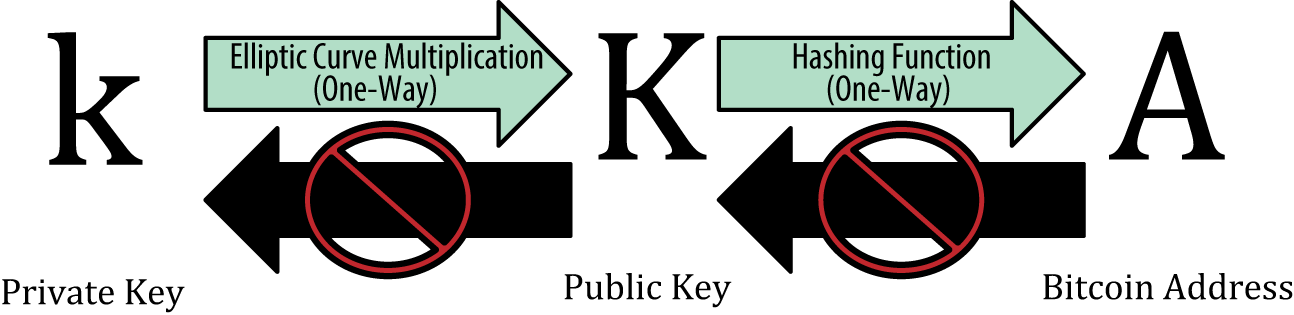
\includegraphics[width=\textwidth]{../../Figures/public_private_key}
                         
  \end{center}
\end{figure}
\begin{itemize}
  \item Private key = Pin number 
  \begin{itemize}
    \item[$\hookrightarrow$] Generate the public key
    \item[$\hookrightarrow$] Sign transaction
  \end{itemize}
  \item Public key =  Bank acccount information
  \begin{itemize}
    \item[$\hookrightarrow$] Verify transaction
  \end{itemize}
\end{itemize}
\end{frame}
\begin{frame}{Unspent transaction}
\begin{figure}
  \begin{center}
      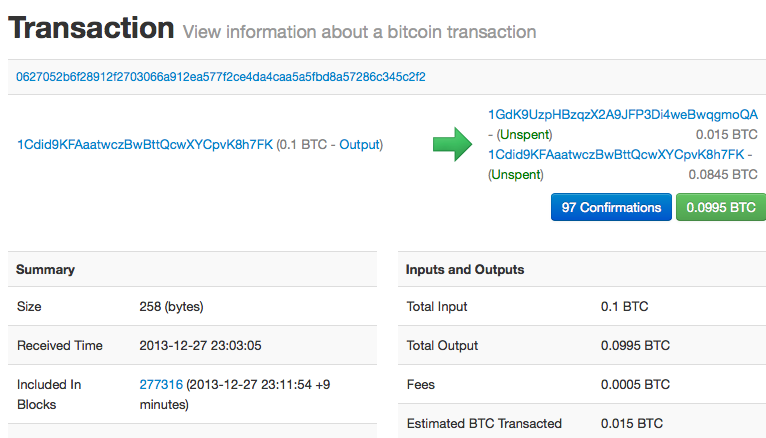
\includegraphics[width=\textwidth]{../../Figures/btc_transaction}
  \end{center}
\end{figure}
\end{frame}
\begin{frame}{User's balance}
\begin{tcolorbox}[enhanced,drop shadow, title= UTXO]
Unspent transaction outputs.
\end{tcolorbox}
The balance of a bitcoin user is the sum of all the UTXO associated to the BTC addresses she controls.
\scriptsize{
\begin{thebibliography}{1}
\bibitem{Antonopoulos2017}
A.~Antonopoulos, {\em Mastering Bitcoin}.
\newblock O'Reilly UK Ltd., July 2017.
\end{thebibliography}  
}
\end{frame}
\begin{frame}[plain]
\begin{figure}
  \begin{center}
      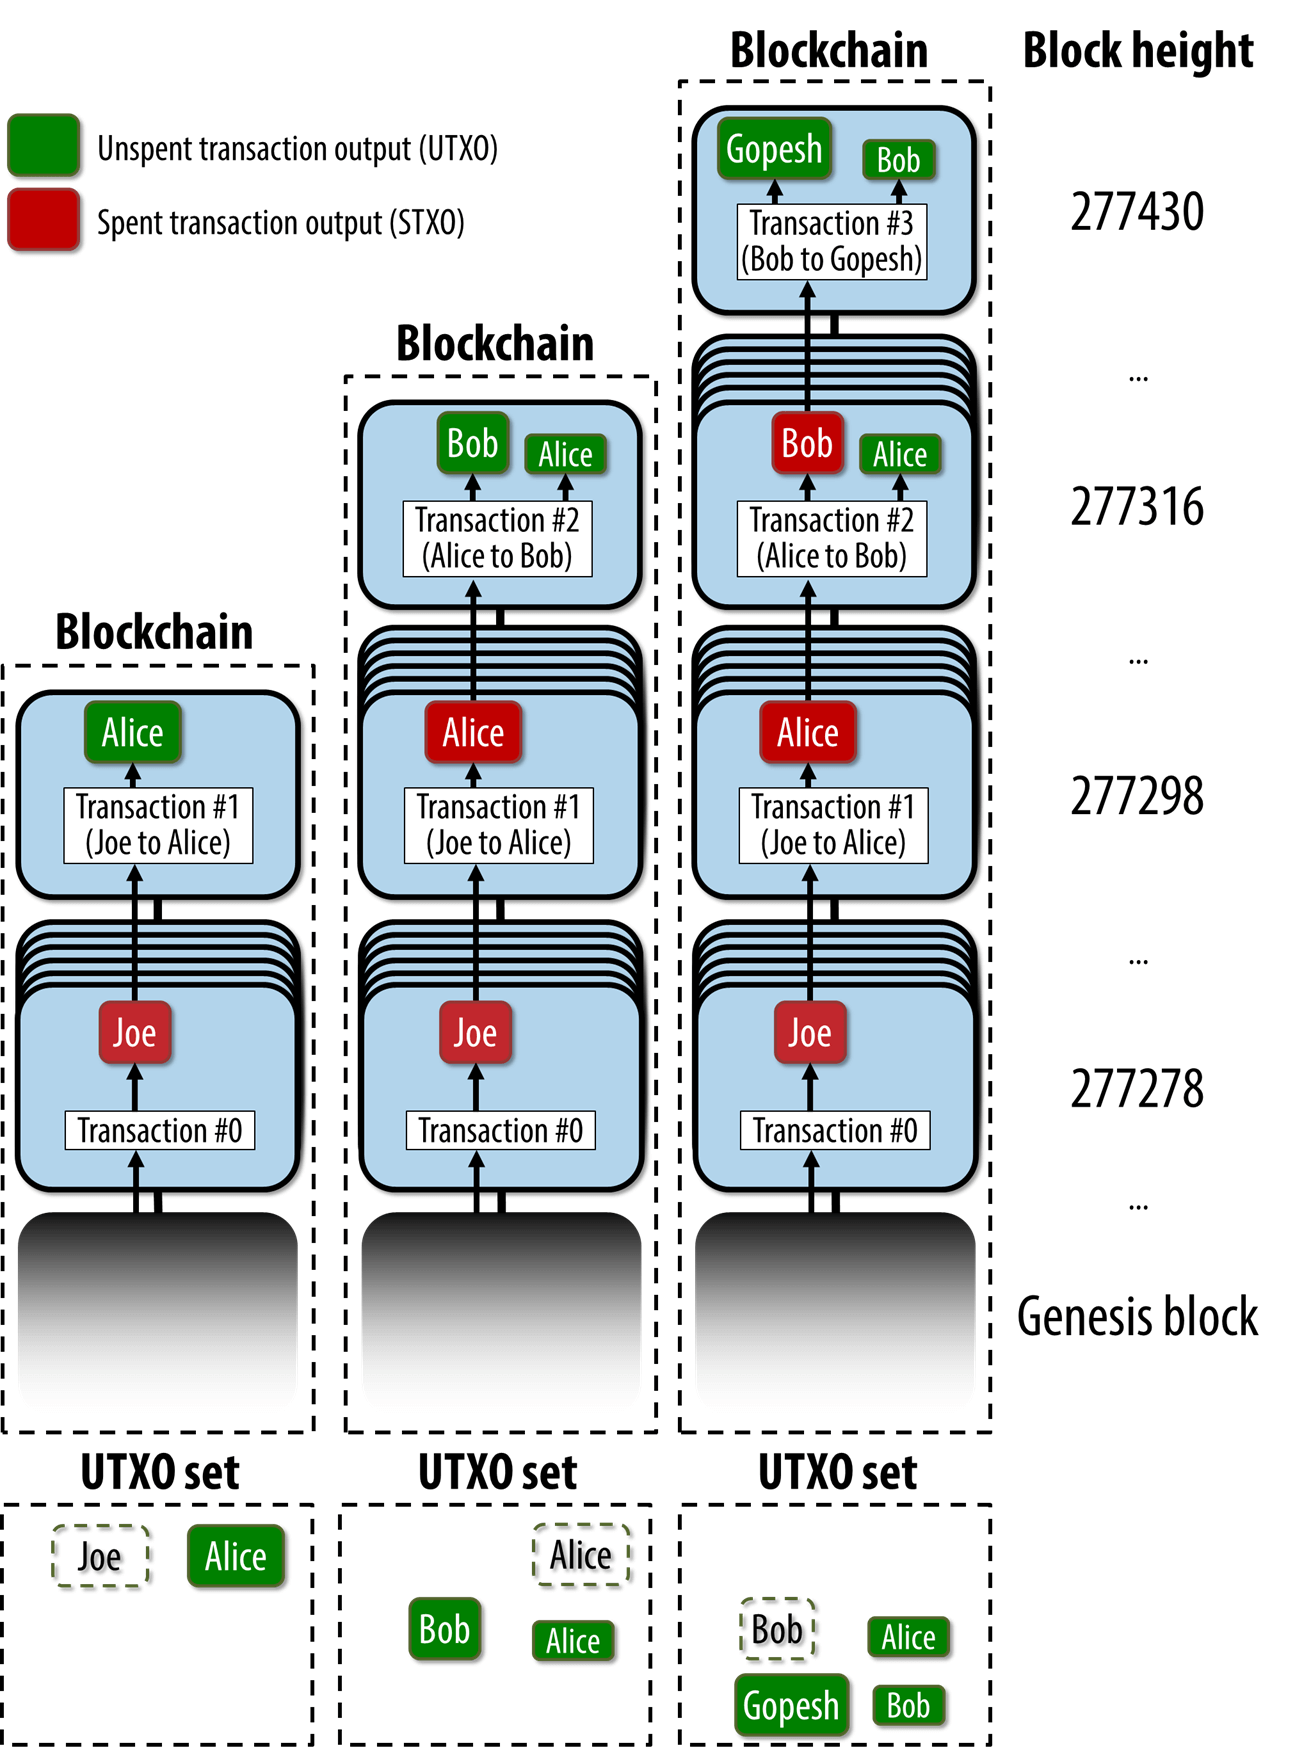
\includegraphics[width=0.7\textwidth]{../../Figures/transaction_tree}
  \end{center}
\end{figure}
\end{frame}
\begin{frame}{Cryptocurrency implementation}
\scriptsize
Blockchain parameters
\begin{itemize}
  \item Consensus protocol (PoW or PoS) 
  \begin{itemize}
    \item[$\hookrightarrow$] \tiny Hash function (SHA-256 for Bitcoin and scrypt for LiteCoin) 
    \item[$\hookrightarrow$] \tiny Hybrid PoW/PoS (PeerCoin)
  \end{itemize}
  \item Block generation time \scriptsize
    \begin{itemize}
    \item[$\hookrightarrow$] \tiny every 10 minutes for Bitcoin 
    \item[$\hookrightarrow$] \tiny every 12 sec for Ethereum
  \end{itemize}
  \item Block finding reward\scriptsize
  \begin{itemize}
    \item[$\hookrightarrow$] \tiny Halved every 210,000 blocks in Bitcoin. It started at 50 BTC, is now 6.25 BTC \url{https://www.bitcoinblockhalf.com/}
  \end{itemize}
  \item Total coin supply\scriptsize
    \begin{itemize}
    \item[$\hookrightarrow$] \tiny 21,000,000 in total for Bitcoin
  \end{itemize}
  \item Transaction fees\scriptsize
      \begin{itemize}
    \item[$\hookrightarrow$] \tiny GAS in Ethereum
  \end{itemize}
\end{itemize}
These choices lead to the creation of multiple cryptocurrencies 
\begin{tcolorbox}[enhanced,drop shadow, title=Examples]
     Bitcoin and AltCoins (Ethereum, LiteCoin, DogeCoin, Ripple... ), see \url{https://en.wikipedia.org/wiki/List_of_cryptocurrencies}
\end{tcolorbox}

\end{frame}

\begin{frame}[plain]
\begin{figure}
\captionsetup[subfigure]{labelformat=empty}
  \begin{center}
   \subfloat[]{

      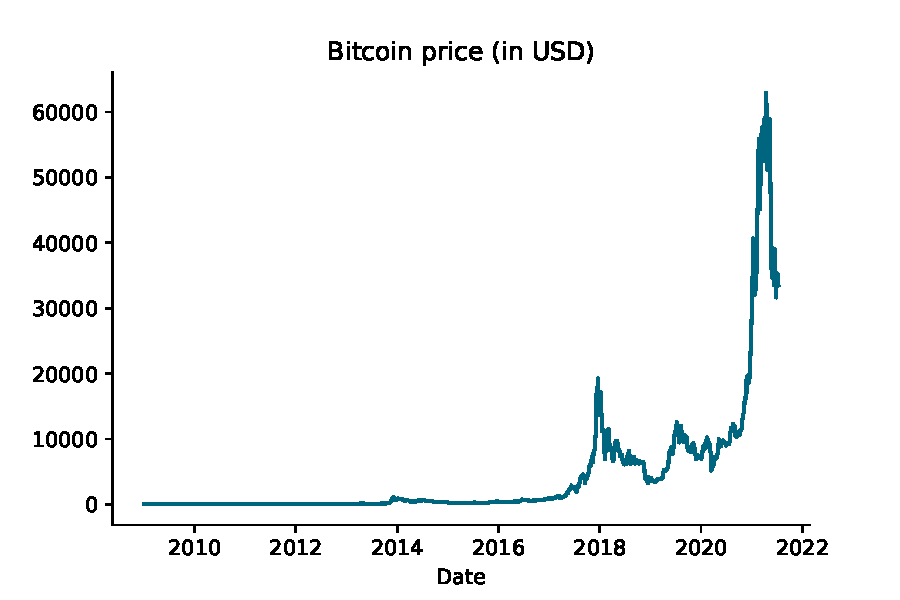
\includegraphics[width=0.42\textwidth]{../../Figures/btc_price}
      \label{sub:QQplot_gamma}
       
                         }
                         \hskip1em
    \subfloat[]{
      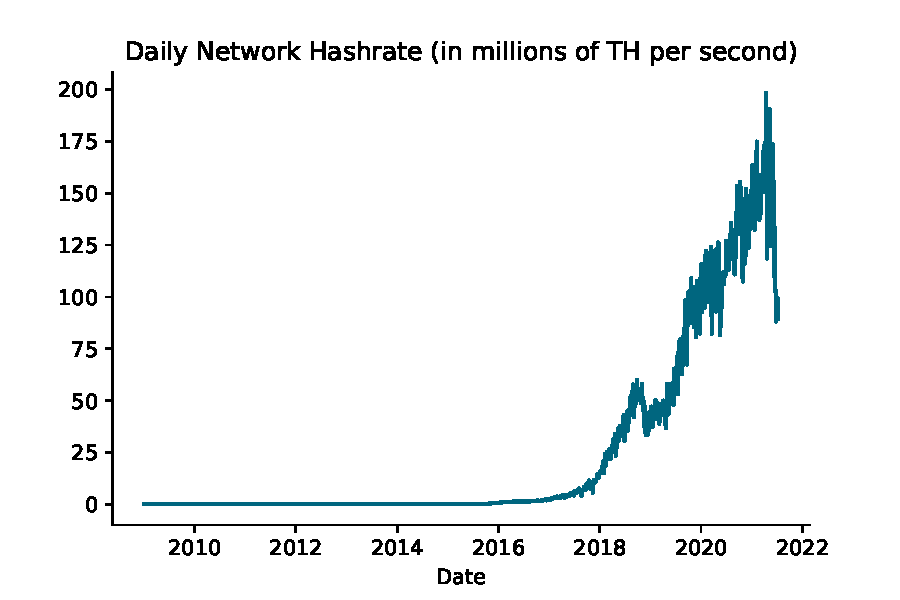
\includegraphics[width=0.42\textwidth]{../../Figures/btc_hahsrate}
      \label{sub:QQplot_weib}
                         }
                         \hskip1em
    \subfloat[]{
      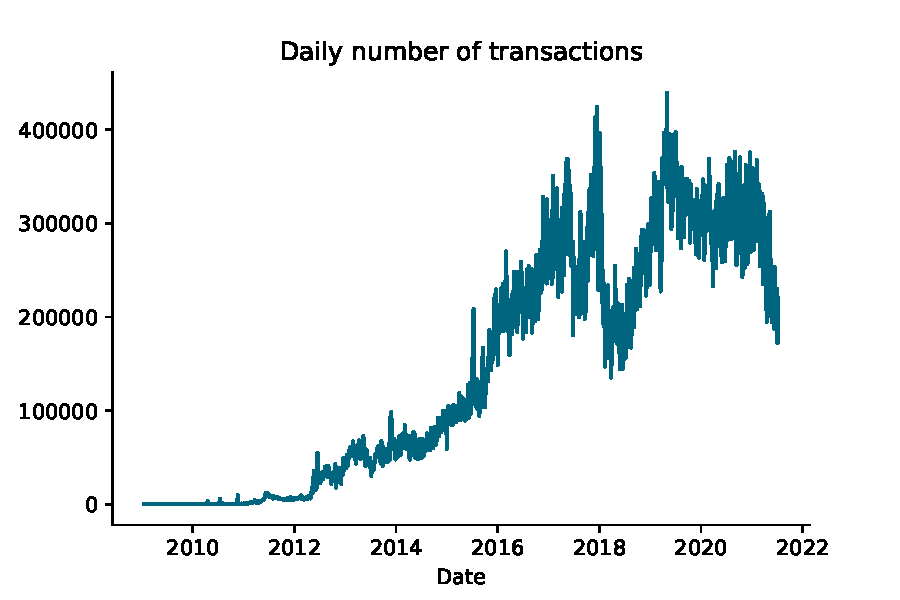
\includegraphics[width=0.42\textwidth]{../../Figures/btc_n_transaction}
      \label{sub:QQplot_lnorm}
                         }
    \subfloat[]{
      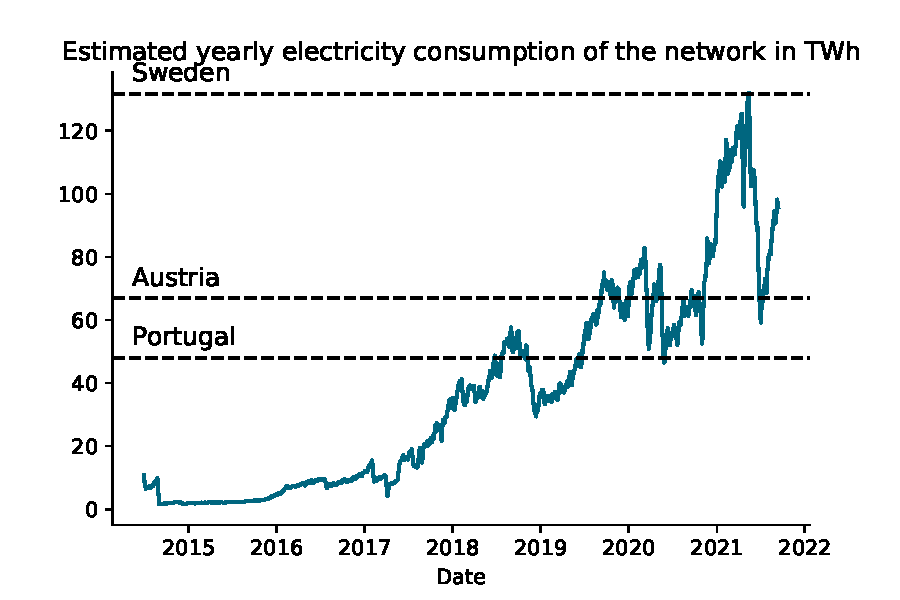
\includegraphics[width=0.42\textwidth]{../../Figures/btc_elec_conso}
      \label{sub:QQplot_pareto}
                         }
    % \caption{Quantile-quantile plots associated to the gamma, Weibull, lognormal and Pareto models fitted to the danish fire insurance loss data using maximum likelihood estimation.}
    % \label{fig:qqplot_weib_lnorm}
  \end{center}
\end{figure}
\blfootnote{\tiny Sources: \url{https://www.blockchain.com/} $\&$ \url{https://cbeci.org/}}
\end{frame}




\begin{frame}{Decentralized application}
The network provide ressources such as
\begin{itemize}
  \item storage
  \item computing power
\end{itemize}
through a smart contract on the ethereum blockchain. 
\vspace{0.3cm}
\begin{tcolorbox}[enhanced,drop shadow, title=GOLEM (\url{https://www.golem.network/})]
    Build a network of idle computers to do paralell computing. 
\end{tcolorbox}
Utility tokens are used to access the service and provision the network ressources.
\begin{tcolorbox}[enhanced,drop shadow, title=Equation of Exchange (Fisher 1911)]
    \[MV = PQ\] 
\end{tcolorbox}
\end{frame}
\begin{frame}{Decentralized finance}
DEFI creates new financial architecture
\begin{columns}
\begin{column}{0.5\textwidth}
\begin{itemize}
\item[+] Non custodial
\item[+] Anonymous
\item[+] Permisionless
\item[+] openly auditable
\end{itemize}
\end{column}
\begin{column}{0.5\textwidth} 
\begin{itemize}
\item[-] Unregulated
\item[-] Tax evasion
\item[-] Fraud
\item[-] Money laundering
\end{itemize} 
\end{column}
\end{columns}
\vspace{0.5cm}
Extends the Bitcoin promises to more complex financial operations
\begin{itemize}
  \item Collateralized lending
  \item Decentralized Exchange Platform
  \item Tokenized assets
  \item Fundraising vehicle (ICO, STO, ...)
\end{itemize}
\vspace{0.3cm}
\scriptsize
\begin{thebibliography}{1}

\bibitem{werner2021sok}
S.~M. Werner, D.~Perez, L.~Gudgeon, A.~Klages-Mundt, D.~Harz, and W.~J.
  Knottenbelt, ``Sok: Decentralized finance (defi),'' 2021.

\end{thebibliography}

\end{frame}
\begin{frame}{Tokenized real-world assets}
\scriptsize
Tokenized version of a real-world, physical asset
\begin{itemize}
  \item Increases the liquidity of certain type of assets
  \item Make certain classes of assets available to the many
  \item Can be used as store of value or collateral
\end{itemize}
These token can be backed by 
\begin{itemize}
  \item fiat currency $\Rightarrow$ stablecoin
  \item commodities like gold \url{https://ekon.gold/}
  \item stocks (security token) that includes voting right and profit sharing mechanism
  \item Art
  \item Digital art (Non Fungible tokens on the Ethereum blockchain)
\end{itemize}
\begin{tcolorbox}[enhanced,drop shadow, title=Central authority]
    This requires a custodian to ensure that the tokens are actually backed by these off-chain assets (except for NFTs).
\end{tcolorbox}

\scriptsize
\begin{thebibliography}{1}

\bibitem{OECD}
OECD, ``The tokenisation of assets and potential implications for financial
  markets,'' tech. rep., 2020.

\end{thebibliography}
\end{frame}
\begin{frame}{Valuation models}
\begin{itemize}
\item Cryptocurrencies are medium of exchange and may be priced via transaction cost model (Beaumol-Tobin and such)

\scriptsize
\begin{thebibliography}{1}
\bibitem{Baumol1952}
W.~J. Baumol, ``The transactions demand for cash: An inventory theoretic
  approach,'' {\em The Quarterly Journal of Economics}, vol.~66, p.~545, nov
  1952.
\bibitem{Schilling2019}
L.~Schilling and H.~Uhlig, ``Some simple bitcoin economics,'' {\em Journal of
  Monetary Economics}, vol.~106, pp.~16--26, oct 2019.
\end{thebibliography}
\normalsize
\item Tokenized asset depends on the real asset that backs the token
\scriptsize
\begin{thebibliography}{1}

\bibitem{Hargrave2019}
J.~Hargrave, N.~Sahdev, and O.~Feldmeier, ``How value is created in tokenized
  assets,'' in {\em Blockchain Economics: Implications of Distributed Ledgers},
  pp.~125--143, {WORLD} {SCIENTIFIC} ({EUROPE}), jan 2019.

\end{thebibliography}
\normalsize
\item Utility tokens
\scriptsize
\begin{thebibliography}{1}

\bibitem{Gan2021}
J.~R. Gan, G.~Tsoukalas, and S.~Netessine, ``Initial coin offerings,
  speculation, and asset tokenization,'' {\em Management Science}, vol.~67,
  pp.~914--931, feb 2021.

\bibitem{Cong2020a}
L.~W. Cong, Y.~Li, and N.~Wang, ``Tokenomics: Dynamic adoption and valuation,''
  {\em The Review of Financial Studies}, vol.~34, pp.~1105--1155, aug 2020.

\end{thebibliography}

\end{itemize}
\end{frame}

\begin{frame}{ICO tuning and timeline}
\begin{enumerate}
  \item ICO period
  \begin{itemize}
    \item \tiny The firm publishes a white paper and set 
    \begin{itemize}
    \item \tiny The token price $\tau$
    \item \tiny The total number of token $m$
    \item \tiny The number of token issued to the investors during the ICO $n\leq m$.
  \end{itemize}
    \item \tiny $s$ among $z>>m$ investors buy token
  \end{itemize}
  \item Production period
  \begin{itemize}
    \item \tiny The firm uses the funds raised $s\tau$ to finance the production of $Q$ units of goods
  \end{itemize}
\item Market period
  \begin{itemize}
    \item \tiny Customers purchase token to meet their needs $D\sim F(.)$
  \end{itemize}
\end{enumerate}
\vspace{0.2cm}
\centering
\begin{tikzpicture}[%
    every node/.style={
        font=\scriptsize,
        % Better alignment, see https://tex.stackexchange.com/questions/315075
        text height=1ex,
        text depth=.25ex,
    },
]
% draw horizontal line   
\draw[->] (0,0) -- (8.5,0);

% draw vertical lines
% \foreach \x in {0,1,...,8}{
%     \draw (\x cm,3pt) -- (\x cm,0pt);
% }

\draw (0 cm,3pt) -- (0 cm,0pt);
\draw (2 cm,3pt) -- (2 cm,0pt);
\draw (4.5 cm,3pt) -- (4.5 cm,0pt);
\draw (7 cm,3pt) -- (7 cm,0pt);
% place axis labels
\node[anchor=north] at (0,0) {\tiny White paper};
\node[anchor=north] at (2,0) {\tiny ICO};
\node[anchor=north] at (2,-0.25) {\tiny starts};
\node[anchor=north] at (4.5,0) {\tiny Production};
\node[anchor=north] at (4.5,-0.25) {\tiny starts};
\node[anchor=north] at (7,0) {\tiny Product};
\node[anchor=north] at (7,-0.25) {\tiny launch};
\node[anchor=south] at (8.5,0) {$t$};

% Draw vertical line
\draw[->] (0,1) -- (0,0.25);
\node[anchor=south] at (0,1) {\tiny Company decides $\tau$ and $n$};
\draw[->] (4.5,1) -- (4.5,0.25);
\node[anchor=south] at (4.5,1) {\tiny Company decides $Q$};

% draw scale above
% \fill[myLightGray] (1,0.25) rectangle (2,0.4);
% \fill[myDarkGray] (2,0.25) rectangle (3,0.4);
% \fill[myDarkRed] (3,0.25) rectangle (4,0.4);
% \fill[myRed] (4,0.25) rectangle (5,0.4);
% \draw[myRed,dashed,thick,-latex] (5.05,0.325) -- (6.05,0.325);

% draw scale below
% \fill[myLightGray] (3,-0.4) rectangle (4,-0.55);
% \fill[myGray] (4,-0.4) rectangle (5,-0.55);
% \fill[myGreen] (5,-0.4) rectangle (6,-0.55);
% \draw[myGreen,dashed,thick,-latex] (6.05,-0.475) -- (7.05,-0.475);

% draw curly braces and add their labels
\draw[decorate,decoration={brace,amplitude=5pt}] (2,0.45) -- (4.25,0.45)
    node[anchor=south,midway,above=4pt] {\tiny Speculators buy tokens};
\draw[decorate,decoration={brace,amplitude=5pt}] (7,0.45) -- (8.5,0.45)
    node[anchor=south,midway,above=4pt] {\tiny Customers buy tokens};
\draw[decorate,decoration={brace,amplitude=5pt}] (4.5,-0.75) -- (2,-0.75)
    node[anchor=north,midway,below=4pt] {\tiny ICO period};
    \draw[decorate,decoration={brace,amplitude=5pt}] (7,-0.75) -- (4.6,-0.75)
    node[anchor=north,midway,below=4pt] {\tiny Production period};
    \draw[decorate,decoration={brace,amplitude=5pt}] (8.5,-0.75) -- (7.1,-0.75)
    node[anchor=north,midway,below=4pt] {\tiny Production period};
\end{tikzpicture}
\tiny
\begin{thebibliography}{1}

\bibitem{Gan2021}
J.~R. Gan, G.~Tsoukalas, and S.~Netessine, ``Initial coin offerings,
  speculation, and asset tokenization,'' {\em Management Science}, vol.~67,
  pp.~914--931, feb 2021.

\end{thebibliography}

\end{frame}
% \begin{frame}{Insights}
% \scriptsize
% \begin{tcolorbox}[enhanced,drop shadow, title=Optimal number of tokens sold $n^\ast$ ]

% The more token the firm sells during the ICO
% \begin{itemize}
%   \item The more money to invest in production
%   \item The less tokens it has to sell in the secondary market
%   \item The less "skin in the game"
%   \item The less it wants to invest in production ex post
% \end{itemize}
% $n^\ast$ resolves the trade off between money now and money later while controlling moral hazard.
% \end{tcolorbox}
% \begin{tcolorbox}[enhanced,drop shadow, title=Optimal token price $\tau^\ast$ ]


% \begin{itemize}
%   \item Price too low: Not enough funds raised
%   \item Price too high: not enough upside for investors
% \end{itemize} 
% \end{tcolorbox}
% Gerry Tsoukalas talk at \\
% \url{https://www.youtube.com/watch?v=E_NT4t4ws8U}
% \end{frame}
\begin{frame}{Decentralized insurance}
\begin{tcolorbox}[enhanced,drop shadow, title=Parametric insurance]
    Compensation if a measurable quantity reaches a threshold 
\end{tcolorbox}
\begin{itemize}
  \item Example: Flight delay insurance
  \begin{itemize}
    \item \url{https://etherscan.io/address/0xdc3d8fc2c41781b0259175bdc19516f7da11cba7}
  \end{itemize}
  \item Use smart contract and off-chain data through oracles
  \item Transparent and automatic
\end{itemize}
\end{frame}
\begin{frame}{Blockchain as a research topic}
\begin{itemize}
  \item Computer science
  \begin{itemize}
  \item Peer-to-peer networks and consensus algorithm
  \item Cryptography and security
  \end{itemize}
  \item Economics  
  \begin{itemize}
  \item Game theory to study the incentive mechanism at play
  \item Nature of the cryptoassets
  \end{itemize}
  \item Operations research  
  \begin{itemize}
  \item Optimization of complex system
  \end{itemize}
  \item Financial math  
  \begin{itemize}
  \item Valuation models for cryptoassets
  \end{itemize}
  \item Machine learning and statistics  
  \begin{itemize}
  \item Open data
  \item Interaction between blockchain users
  \item (Social) network analysis
  \item Clustering of public keys and addresses in the bitcoin blockchain.
  \end{itemize}
\end{itemize}

\end{frame}


% \begin{frame}
% \bibliography{../../blockastics}
% \bibliographystyle{ieeetr}
% \end{frame}

\end{document}
